\documentclass[12pt,report,final,twoside,accentcolor=tud9b,bigchapter]{tudreport}


\usepackage[utf8]{inputenc}


\usepackage{chngcntr}
\counterwithout{equation}{chapter}
\usepackage{pdfpages}
\usepackage{listings}
\usepackage{booktabs}
\usepackage{hyperref}
\usepackage{ngerman}
\usepackage[ngerman,nameinlink,noabbrev]{cleveref}
\usepackage[ngerman]{babel}
\usepackage[onehalfspacing]{setspace}
\usepackage[numbers]{natbib}
\usepackage{amsthm}
\usepackage{amsmath}
\usepackage{mathtools}
\usepackage{enumitem}
\usepackage{pgfplots}
\usepackage{filecontents}
\usepackage{siunitx}
\usepackage{libertine} 
\usetikzlibrary{decorations.pathreplacing}
\usetikzlibrary{intersections}
\usetikzlibrary{circuits.ee.IEC}
\usetikzlibrary{patterns}
\usepackage{nicefrac}
\pgfplotsset{compat=newest}


\newcommand{\Uin}{U_\textrm{in}} 
\newcommand{\Uout}{U_\textrm{out}}
\newcommand{\Usin}{U_\mathrm{sin}}  


% Default fixed font does not support bold face
\DeclareFixedFont{\ttb}{T1}{txtt}{bx}{n}{12} % for bold
\DeclareFixedFont{\ttm}{T1}{txtt}{m}{n}{12}  % for normal

% Custom colors
\usepackage{color}
\definecolor{deepblue}{rgb}{0,0,0.5}
\definecolor{deepred}{rgb}{0.6,0,0}
\definecolor{deepgreen}{rgb}{0,0.5,0}


% Python style for highlighting
\newcommand\pythonstyle{\lstset{
language=Python,
basicstyle=\ttm,
otherkeywords={self},            % Add keywords here
keywordstyle=\ttb\color{deepblue},
emph={MyClass,__init__},          % Custom highlighting
emphstyle=\ttb\color{deepred},    % Custom highlighting style
stringstyle=\color{deepgreen},
frame=tb,                        % Any extra options here
showstringspaces=false            %
}}


% Python environment
\lstnewenvironment{python}[1][]
{
\pythonstyle
\lstset{#1}
}
{}

% Python for external files
\newcommand\pythonexternal[2][]{{
\pythonstyle
\lstinputlisting[#1]{#2}}}
\bibliographystyle{natdin}

% Python for inline
\newcommand\pythoninline[1]{{\pythonstyle\lstinline!#1!}}


\newcommand{\ra}[1]{\renewcommand{\arraystretch}{#1}}

\pgfplotsset{grid style={dashed,gray}}
\pgfplotsset{minor grid style={dashed,red}}
\pgfplotsset{major grid style={dashed,gray}}


\begin{document}

~\\
\begin{tabular}{p{.178\linewidth}p{.50\linewidth}p{.3\linewidth}}
  \multicolumn{2}{p{.678\linewidth}}{
    \fontfamily{\sfdefault}\fontseries{mb}
        \vspace*{-0.2em}
        % ***** change title here
       % \LARGE Projektseminar Beschleunigertechnik
        % ***** change title here
        }
  &
%\raisebox{-.8\height}{\includegraphics[width=.8\linewidth]{Images/TUDLogo.pdf}}

\end{tabular}
\vspace*{1.5em}
\vskip\medskipamount
\leaders\vrule width \textwidth\vskip0.4pt
\vskip\medskipamount
\nointerlineskip
% comment the following lines if no authors are given
% begin comment
\noindent
\begin{minipage}{0.8\textwidth}
\begin{flushleft}
Denys Bast, Armin Galetzka\\
Institut f\"{u}r Theorie Elektromagnetischer Felder
\end{flushleft}
\end{minipage}
\begin{minipage}{0.19\textwidth}
\begin{flushright}
%\includegraphics[width=0.25\textwidth]{Images/TEMF-Logo06f.png}
\end{flushright}
\end{minipage}

\vskip\medskipamount
\leaders\vrule width \textwidth\vskip0.4pt
\vskip\medskipamount
\nointerlineskip
% end comment
\vspace*{1em}

  \title{Projektseminar Beschleunigertechnik}
  \maketitle

\tableofcontents
\chapter{Abstract}
Das breitbandige Bestimmen der Übertragungsfunktion eines unbekannten
Systems ist mit Methoden wie dem Sinus Sweep aufwendig und zeitintensiv.
Pseudorauschen ist eine Möglichkeit, schnell und effizient den Frequenzgang eines Systems in einem breiten Spektrum zu bestimmen. Im Rahmen dieses Seminars wurde ein Python Tool zur automatisierten Messung der Übertragungsfunktion eines Kavitätensystems implementiert und erfolgreich getestet. Als Pseudo-Rauschsignal wurde ein MLBS (\textit{maximum length binary sequence}) Signal verwendet. Der Vergleich der neuen Methode mit dem Sinus Sweep ergab eine hohe Übereinstimmung der Übertragungsfunktion bei gleichzeitiger Reduktion der Messdauer von 30 Minuten auf 42 Sekunden.


\chapter{Einführung der Problemstellung} \label{cha:einfuehrung}

Für das Großprojekt FAIR werden von der Organisationseinheit SIS - Abteilung Ring RF des GSI Helmholtzzentrums für Schwerionenforschung Barrier-Bucket Systeme entworfen. Diese Systeme dienen der longitudinalen Manipulation von Teilchenstrahlen. Dazu müssen am Gap der Kavität einzelne sinusförmige Spannungspulse erzeugt werden. Das dafür geplante System besteht aus Signalgenerator, Verstärker und Kavität. 
\begin{figure}[htb] 
\begin{minipage}[t]{0.48\linewidth}     
  \centering
  \includegraphics[scale=0.2]{Images/Kavitaeteinaus2.png}  
  \caption{Kavität}
  \label{fig:Kavitaet}
\end{minipage}
  \hfill
\begin{minipage}[t]{0.48\linewidth}     
  \centering
\begin{tikzpicture}[thick]
\draw[fill=white] (-0.06,0.2) circle (2pt)
                  (-0.06,1.8) circle (2pt)
                  (4.06,0.2) circle (2pt)
                  (4.06,1.8) circle (2pt);               
  \draw (0,0.2) -- (1,0.2);
  \draw (0,1.8) -- (1.0,1.8);
  \draw[->] (-0.2,1.7) -- (-0.2,0.3);
  \draw (-0.2,1) -- (-0.2,1.1) node[left] {$\underline{U}_\mathrm{in}$};
  \draw (4,1.8) -- (3,1.8);
  \draw (4,0.2) -- (3,0.2);
  \draw[->] (4.2,1.7) -- (4.2,0.3);
  \draw (4.2,1) -- (4.2,1.1) node[right] {$\underline{U}_\mathrm{out}$};
  \draw (1,0) rectangle	(3,2);
  \node at (2,1) {Zweitor};
\end{tikzpicture}
\caption{Beliebiges Zweitor}
\label{fig:zweitor}
\end{minipage}
\end{figure}
Für ausreichend kleine Eingangssignale verhält sich das System linear. Das Verhalten des Systems kann dann mathematisch durch den Frequenzgang $\underline{H}(\omega)$ beschrieben werden. Abbildung \ref{fig:Kavitaet} zeigt die auszumessende Kavität mit den Spannungen $\underline{U}_\mathrm{in}$, $\underline{U}_\mathrm{out,1}$ und $\underline{U}_\mathrm{out,2}$. Die Spannung $\underline{U}_\mathrm{in}$ liegt an den Einkopplungsschleifen an. Die Ausgangsspannungen liegen am Gap an. Messtechnisch ist es einfacher das Ausgangssignal an zwei Stellen zu erfassen. Die gesamte Ausgangsspannung ist gegeben durch
\begin{equation}
\underline{U}_\mathrm{out} = \underline{U}_\mathrm{out,1} - \underline{U}_\mathrm{out,2}.
\end{equation}
Eine abstraktere Betrachtung des Problems führt auf die Darstellung durch ein Zweitor, siehe Abbildung \ref{fig:zweitor}.
Wenn der Frequenzgang bekannt ist, kann im Frequenzbereich (Fouriertransformation) zu einem Eingangssignal $\underline{U}_{\mathrm{in}}$ das Ausgangssignal $\underline{U}_{\mathrm{out}}$ mit 
\begin{equation}
\underline{U}_{\mathrm{out}}(\omega)=\underline{H}(\omega)\cdot \underline{U}_{\mathrm{in}}(\omega)
\label{eq:UF1}
\end{equation}
bestimmt werden. Durch Umformen von Gleichung \eqref{eq:UF1} auf \begin{equation}
\underline{U}_{\mathrm{in}}(\omega)=\underline{U}_{\mathrm{out}}(\omega)\cdot \underline{H}(\omega)^{-1},
\label{eq:UF2}
\end{equation}
lässt sich aus einem bekannten Ausgangssignal das Eingangsignal berrechnen. \cite{Frey2015}

Ziel ist es, ein Einzelsinus-Signal am Ausgang zu erzeugen. Für eine Periodendauer von $T_{\mathrm{BB}}$ ist der Einzelsinus wie folgt definiert. \cite{Harzheim2017}

\begin{equation}
   \Usin(t) =
   \begin{cases}
     -\widehat{U} \cdot \sin \left(\frac{2 \pi}{T_{\mathrm{BB}}}t\right) & \text{für } -\frac{T_{\mathrm{BB}}}{2} \textless t \textless \frac{T_{\mathrm{BB}}}{2} \\
     0 & \text{sonst} \\
     
   \end{cases}
\end{equation}
Abbildung \ref{fig:Einzelsinus} zeigt ein solches Einzelsinus Signal.
\begin{figure}[h!]
\centering
    \begin{tikzpicture}
\begin{axis}[grid=both, xlabel={$t/T_{\textrm{BB}}$},
ylabel={$\Usin(t)$},                        ytick={-1,1},
                        yticklabels={$-\widehat{U}$,$\widehat{U}$},
                        xtick={-4,-2,0,2,4},
                        xticklabels={-2,-1,0,1,2}]
\addplot[blue, thick] table [ x expr={\thisrowno{0}}, y
expr={\thisrowno{1}}, col sep=semicolon] {Plots/Einzelsinus.csv};
\end{axis}
\end{tikzpicture}
\caption{Einzelsinus}
  \label{fig:Einzelsinus}
\end{figure}
Das Spektrum des Einzelsinus setzt sich aus zwei verschobenen si-Funktionen zusammen. Abbildung \ref{fig:SpektrumSinus} zeigt die Fouriertransformierte des Einzelsinus der Amplitude $\widehat{U}$ und der Kreisfrequenz $\omega_{\mathrm{BB}}$. Ein idealer Einzelsinus beinhaltet also beliebig hohe Frequenzen. Da dies technisch nicht realisierbar ist, kommt es zu sogenannten Überschwingern vor und hinter dem Sinuspuls. Diese sollen im Bereich von $2,5\,\mathrm{\%}$ der Amplitude $\widehat{U}$ liegen. \cite{Frey2015a, Harzheim2017, Jatta2013, TechCoSIS}
\begin{figure}[htb]
\centering
\begin{tikzpicture}
	  \begin{axis}[legend entries={$\Usin (\omega)$},
	               x=1.1cm,
	               grid=both,
	               legend pos=south east,
	               legend style={row sep=1.8pt},
	               xmin=-6,xmax=6,
	               ytick={-1,0,1},
	               yticklabels={$-\nicefrac{\widehat{U}\pi}{\omega_\mathrm{BB}}$,0,$\nicefrac{\widehat{U}\pi}{\omega_\mathrm{BB}}$},
	               xlabel={$\omega/\omega_\mathrm{BB}$},
				   ylabel={Spektraldichte in $\SI{}{\volt\second}$}]
	    %\addplot[color=blue, thick] table [x expr={\thisrowno{0}},
 		%						            y expr={\thisrowno{1}}, 
 		%						   col sep=semicolon] {Plots/EinzelsinusSpektrum.csv};
 		%\addplot[color=red, thick] table [x expr={\thisrowno{0}},
 		%						      y expr={\thisrowno{2}}, 
 		%						   col sep=semicolon] {Plots/EinzelsinusSpektrum.csv};
        \addplot[color=black, very thick] table [x expr={\thisrowno{0}},
 								   y expr={\thisrowno{3}}, 
 								   col sep=semicolon] {Plots/EinzelsinusSpektrum.csv};
	  \end{axis}
	\end{tikzpicture}
      \caption{Frequenzspektrum eines Einzelsinus der Amplitude $\widehat{U}$ und der Kreisfrequenz $\omega_{\mathrm{BB}}$ \citep{Harzheim2017}}
      \label{fig:SpektrumSinus}
\end{figure}

Die Ausgangspannung in Gleichung \ref{eq:UF2} ist damit gegeben durch $\underline{U}_\mathrm{out}(\omega)=\Usin(\omega)$. Wird der Frequenzgang gemessen, kann mit Gleichung \ref{eq:UF2} das Eingangssignal berechnet werden, das angelegt werden muss, um einen Einzelsinus am Ausgang des Systems zu erhalten. \cite{Frey2015, Harzheim2017}


Es existiert ein intern entwickeltes Programm, das bei bekannter Übertragungsfunktion ein solches vorverzerrtes Signal erzeugt \cite{Gross2013}. Bisher wird die Übertragungsfunktion mit Hilfe eines sinusförmigen Kleinsignal-Sweeps im Frequenzbereich von $10\, \mathrm{kHz}$ bis $80\, \mathrm{MHz}$ gemessen. Um sicherzustellen, dass sich das System im eingeschwungenen Zustand befindet, muss der Sweep ausreichend langsam durchgeführt werden. Dies führt zu einer langen und aufwändigen Prozedur der Messung. \cite{Frey2015}

Ziel dieses Projektseminars ist es, ein Python-Tool zu entwickeln, mit dessen Hilfe die Messung des Frequenzganges des Systems automatisiert und zeiteffizient durchgeführt werden kann. 

Weißes Rauschen regt gleichzeitig breite Frequenzbereiche an und eignet sich daher als Eingangssignal anstelle des Sweeps. So kann mit einem Messdurchgang die Übertragungsfunktion für alle interessanten Frequenzen bestimmt werden. Dadurch kann die Messung sehr viel schneller durchgeführt werden. \citep{skript}

\chapter{Pseudorauschen} \label{cha:rauschen}
Pseudo-Rauschsignale sind digital erzeugte Folgen von Zufallszahlen, die das Verhalten und die Eigenschaften von weißem Rauschen nachbilden sollen. Im Folgenden wird erläutert, was Pseudo-Rauschsignale auszeichnet und was deren Eigenschaften sind. Anschließend wird dargelegt wie Pseudorauschen erzeugt werden kann. Im Anschluss wird die für dieses Projektseminar erstellte Implementierung in Python vorgestellt. \citep{skript}



\section{Erzeugung von Pseudorauschen}
Weißes Rauschen kann als Folge identisch verteilter, unabhängiger Zufallsvariablen betrachtet werden. Damit beschreibt es einen stochastischen Prozess, der mittelwertfrei und in sich unkorreliert ist. Außerdem besitzen dessen Variablen eine gleiche Verteilung. \citep{skript, Nachrichtentechnik}

Um digitale Rauschsignale als Eingangssignale verwenden zu können, müssen diese
am Digitalrechner generiert werden. Dies geschieht über sogenannte
Pseudo-Zufallszahlen, deren Eigenschaften bezüglich Verteilung,
Mittelwert und Korrelation die von weißem Rauschen nachbilden. Im
Folgenden soll $T_{\mathrm{ns}}$ die Taktzeit des Rauschens und
$T_\mathrm{s}$ die Abtastzeit der Messung bezeichnen.
\begin{figure}[h!]
  \centering
      \includegraphics[scale=0.35]{Images/AutokorrelationPBRS.PNG}
      \caption{Autokorrelationsfunktion eines PBRS mit Taktzeit
$T_{\mathrm{ns}}$ und Länge $N_\mathrm{N}$ \citep{skript}}
      \label{fig:AutoPBRS}
\end{figure}
Wird eine periodische Folge von binären Pseudo-Zufallszahlen erzeugt und
hat diese eine Autokorrelationsfunktion nach Abbildung \ref{fig:AutoPBRS},
wird dieses Signal als Pseudo-Binär-Zufallsprozess (\textit{PBRS -
pseudo random binary signal}) bezeichnet. Eine binäre Zufallszahl kann lediglich zwei Werte annehmen. Es werden die Zahlen $0$ und $1$ zufällig gezogen, wobei beide die gleiche Wahrscheinlichkeitsverteilung besitzen. Abbildung \ref{fig:probDen} zeigt die diskrete Verteilung der Zufallsvariablen. Die erzeugten Zufallszahlen werden am PC berechnet und sind reproduzierbar, erfüllen aber wichtige Kriterien echter Zufallszahlen. \cite{MC}
\begin{figure}[h!] 
\begin{minipage}[t]{0.48\linewidth}     
  \centering
\begin{tikzpicture}
\begin{axis}[xmin=-0.2,xmax=1.2,
			 xlabel={Registerwert},
			 ylabel={Relative Häufigkeit},
			 ymin=0,ymax=1,
			 xtick={0,1},
	         ytick={0,0.5,1},
	         grid=both]
	\draw[red, ultra thick] (0,0)--(0,0.5)node[circle,fill,draw,scale=.3]{};
	\draw[red, ultra thick] (1,0)--(1,0.5)node[circle,fill,draw,scale=.3]{};
\end{axis}
\end{tikzpicture}
\caption{Diskrete Verteilung der Zufallsvariablen}
\label{fig:probDen}
\end{minipage}
  \hfill
\begin{minipage}[t]{0.47\textwidth}
	\ra{1.2}
		\centering
		\raisebox{\depth}{\begin{tabular}{@{}lll@{}}
\toprule
Bits & $N_\mathrm{n}$ & Rückführung\\
\midrule
6 & 63 & $0 \oplus 5$\\
7 & 127 & $0 \oplus 6$\\
8 & 255 & $0 \oplus 1 \oplus 6 \oplus 7$\\
9 & 511 & $3 \oplus 8$\\
10 & 1023 & $2 \oplus 9$\\
11 & 2047 & $1 \oplus 10$\\
\bottomrule
\\
\\
\end{tabular}}
		\captionof{table}{Rückgeführte Bit zum Schieben des Registers}
		\label{tab:MLBS}
\end{minipage}
\end{figure}

Eine Möglichkeit ein solches Signal zu erzeugen, ist die MLBS
(\textit{maximum length binary sequence}). Dabei wird ein
Schieberegister verwendet, um die Folge mit den gewünschten
Eigenschaften zu erzeugen. Das Schieberegister wird mit zufälligen Zahlenwerten aus $\{0,1\}$ initialisiert, wobei mindestens ein Bit den Zustand $1$ haben muss. Daher ergibt sich für ein Schieberegister mit $b$ Bit eine Folge der Länge 
\begin{equation}
N_\mathrm{n} = 2^b-1.
\end{equation}
Abbildung \ref{fig:RegMLBS} zeigt ein solches Schieberegister für $b=7$ Bit.
\begin{figure}[h!]
  \centering
      \includegraphics[scale=0.5]{Images/RegisterMLBS.PNG}
      \caption{Schieberegister zur Erzeugung eines MLBS der Länge
$N_N=127$ \citep{skript}}
      \label{fig:RegMLBS}
\end{figure}
Das Schieberegister gibt mit jedem Takt ein Bit 0 oder 1 aus, wobei jedes einer Spannung $u_0$ oder $-u_0$ zugeordnet wird. Das erzeugte Signal hat also nur zwei diskrete Spannungsniveaus. 
Es müssen mindestens zwei Bit zurückgeführt werden, um ein MLBS erzeugen
zu können. Eines der beiden Bit muss das letzte sein. Welches Bit noch
zurückgeführt wird, hängt von der Länge des Schieberegisters ab. Bei 6
und 7 Bit wird jeweils das erste und das letzte Bit zurückgeführt. Die Kombination der
zurückgeführten Bits ist in Tabelle \ref{tab:MLBS} für verschiedene
Längen $b$ des Schieberegisters gezeigt.

Für ein solches Signal lässt sich die Fourier-Reihe bestimmen, deren
absolute Koeffizienten gegeben sind durch
\begin{equation}
|u_\ell| \le \left\{\begin{array}{ll} \frac{u_0}{N_\mathrm{n}} & \ell=0,
\\
u_0\frac{\sqrt{N_\mathrm{n}+1}}{N_\mathrm{n}}\left|\frac{\sin\left(\frac{\ell
\pi}{N_\mathrm{n}}\right)}{\frac{\ell \pi}{N_\mathrm{n}}}\right| & \ell
>0. \\
          \end{array}\right.
\label{eq:fourieKoef}
\end{equation}
Die Dämpfung der Koeffizienten ist durch die einhüllende si-Funktion beschrieben.
Für $\ell=N_\mathrm{n}$ gilt für Gleichung \eqref{eq:fourieKoef}
\begin{equation}
|u_{N_\mathrm{n}}|=u_0
\frac{\sqrt{N_\mathrm{n}+1}}{N_\mathrm{n}}\left|\frac{\sin\left(\pi\right)}{\pi}\right|=0.
\end{equation}
Der Fourier Koeffizient verschwindets bei $\ell=N_\mathrm{n}$. Durch
die Dämpfung ist die Anregung ab einem gewissen Frequenzbereich nicht
mehr hoch genug. Abbildung \ref{fig:FourierMLBS} zeigt die Fourier Koeffizienten über $\ell$.
\begin{figure}[h!]
    \begin{tikzpicture}
\begin{axis}[grid=both, xlabel={$\ell$},
                        ylabel={$\nicefrac{|u_\ell|}{u_\mathrm{0}}$},
                        xmin=0,xmax=255,
                        x=0.06cm]
\addplot+[ycomb] plot table[x index=0, y index=1, col sep=semicolon]{Plots/fourierMLBS.csv};
\end{axis}
\end{tikzpicture}
\caption{Fourier Koeffizienten, bei $\ell =N_\mathrm{n}$ wird der Koeffizient das erste mal $0$ }
  \label{fig:FourierMLBS}
\end{figure}
Die Wahl der Taktzeit $T_{\mathrm{ns}}$ des erzeugten Rauschsignals,
also die Zeit zwischen zwei Pulsen, bestimmt die höchste Frequenz $f_\mathrm{max}$ die gut angeregt wird. Einen Anhaltswert dafür
liefert die Formel $T_{\mathrm{ns}}=0,4/f_{\mathrm{max}}$. Die Frequenz $f_\mathrm{max}$ ist dann mit ungefähr $\SI{-3}{\decibel}$ gedämpft. Der verwendete Funktionsgenerator erwartet eine Sampling Rate. Diese ist gegeben durch $f_\mathrm{ns}=1/T_{\mathrm{ns}}=2.5f_{\mathrm{max}}$.

Zusammen mit der Gesamtlänge $N_\mathrm{n}$ ergibt sich die
Periodendauer des Signals zu $T_\mathrm{p}=N_\mathrm{n}T_\mathrm{ns}$
beziehungsweise die Frequenz zu $f_\mathrm{p}=1/T_\mathrm{p}$. Wie in
Kapitel \ref{cha:einfuehrung} beschrieben, soll eine
Übertragungsfunktion bestimmt werden.
Dazu wird das Signal in den Frequenzbereich transformiert. Für den Fall
von diskreten Daten im Zeitbereich, findet die Diskrete
Fourier-Transformation Anwendung (DFT). Die Auflösung der DFT ist durch
die Frequenz $f_\mathrm{p}$ bestimmt. Das Signal enthält nur vielfache der Frequenz $f_\mathrm{p}$, folglich werden nur vielfache dieser Frequenz berechnet. Ist die Auflösung für die Anwendung nicht
ausreichend fein, muss die Anzahl an Bits erhöht werden.
Zusammenfassend lässt sich sagen:
\begin{enumerate}
\item[$\bullet$] $f_\mathrm{ns}$ ist nach der Frequenz auszulegen, die noch gut angeregt werden soll und gegeben durch
\begin{equation}
f_\mathrm{ns} = 2.5f_{\mathrm{max}}.
\end{equation}
\item[$\bullet$] Die Anzahl der Bits $b$ ist nach der notwendigen Frequenzauflösung $f_\mathrm{p}$ auszulegen und ist bestimmt durch
\begin{equation}
b = \left\lceil \ln\left(2.5\frac{f_\mathrm{max}}{f_\mathrm{p}}+1\right)\ln(2)^{-1} \right\rceil \in \mathbb{N},
\end{equation}
mit der Aufrundungsfunktion $n=\lceil x \rceil$ definiert als $x \le n <x+1$ mit $n \in \mathbb{N}$.
\end{enumerate}
Bei der Messung des MLBS Signals ist darauf zu achten, dass immer
vollständige Perioden erfasst werden. Außerdem muss für die Berechnung
der Fourierkoeffizienten aus einer Messung mit einer entsprechend hohen
Frequenz abgetastet werden, sodass diese ausreichend genau berechnet werden können. Für $T_\mathrm{s} = T_{\mathrm{ns}}$, wobei $T_\mathrm{s}$ die Abtastzeit der Messung ist, liegt der
Fehler der berechneten Koeffizienten in der Größenordnung der
Referenzwerte. Es handelt sich trotzdem um eine sehr gute Näherung für
weißes Rauschen. Bei $T_\mathrm{s} = 0,1 \cdot T_{\mathrm{ns}}$ befindet
sich der Fehler im Bereich bis zu $10\,\%$ und bei $T_\mathrm{s} = 0,01
\cdot T_{\mathrm{ns}}$ bei $1\,\%$. \citep{skript, Isermann2011, Pintelon2001, Golomb2006}
\begin{figure}[h!]
    \begin{tikzpicture}
\begin{axis}[grid=both, xlabel={$t/T_{\textrm{ns}}$},
                        ylabel={$U(t)$},
                        x=0.08cm,
                        ytick={-0.5,0.5},
                        yticklabels={$-U_0$,$U_0$},
                        xtick={0,37.40,74.8,112.2,149.6,187},
                        xticklabels={0,25,50,75,100,125},
                        minor xtick={190},
                        xmin=0,xmax=200]
\addplot[blue, thick] table [ x expr={\thisrowno{0}}, y
expr={\thisrowno{1}}, col sep=semicolon] {Plots/MLBS.csv};
\end{axis}
\end{tikzpicture}
\caption{MLBS Signal für $n=7$ bits mit dem Startregister
$[1~1~0~1~0~1~1]$.  Die rote Linie markiert das Ende der Periode bei
$N=127$.}
  \label{fig:MLBS}
\end{figure}

\section{Implementierung in Python}
Da in der Abteilung Ring RF bereits mit Python gearbeitet
wird, soll die hier entwickelte Software zur Bestimmung der
Übertragungsfunktion ebenfalls als Python Code implementiert werden.
Abbildung \ref{fig:pythonMLBS} zeigt den Code zur Erzeugung eines MLBS Signals. Dieser implementiert ein Schieberegister mit wahlweise 6, 7, 8, 9 bzw. 10 Bit. Abbildung \ref{fig:MLBS} zeigt das erzeugte Pseudo-Rauschsignal
im Zeitbereich für das Startregister ${[1 1 0 1 0 1 1]}$. Es wird ein
Signal mit 7 Bit und somit einer Länge von 127 erstellt. Zur Validierung des erzeugten Signals wird die Autokorrelation bestimmt.
Abbildung \ref{fig:correlation} zeigt diese für eine Periode. Es ist zu
erkennen, dass diese mit den theoretischen Erwartungen (Abbildung
\ref{fig:AutoPBRS}) übereinstimmt.
\begin{figure}[h!]
\centering
    \begin{tikzpicture}
\begin{axis}[grid=both, xlabel={$t/T_{\textrm{ns}}$},
ylabel={$\textrm{Cov}\left[U(t_1),U(t_2)\right]$},
                        ytick={0,31.75},
                        yticklabels={0,$U_0^2$}]
\addplot[blue, thick] table [ x expr={\thisrowno{0}}, y
expr={\thisrowno{1}}, col sep=semicolon] {Plots/correlation.csv};
\end{axis}
\end{tikzpicture}
\caption{Autokorrelation einer Periode des Signals. Nur bei t=0, also
dem unverschobenen Signal, ist eine Korrelation feststellbar.}
  \label{fig:correlation}
\end{figure}
\begin{figure}
\begin{singlespace}
\pythonexternal{MLBS.py}
\end{singlespace}
\caption{MLBS Implementierung in Python}
\label{fig:pythonMLBS}
\end{figure}



\chapter{Algorithmus} \label{sec:algorithmus}
Im folgenden Kapitel wird der erstellte Algorithmus und die Implementierung für die automatische Ermittlung der Übertragungsfunktion vorgestellt.

Die Implementierung des Pseudorauschens und die Auswertung der Übertragungsfunktion ist abhängig von den verwendeten Komponenten.

\section{Software und Ansteuerung}
Das Signal wird mit einem zweikanaligen Funktionsgenerator \textit{Keysight 33600A Series Waveform Generator}, im Folgenden als AWG (\textit{arbitary wave generator}) bezeichnet, erzeugt. Zum Messen wird ein digitales Oszilloskop vom Typ \textit{Tektronix TDS 5054 Digital Phosphor Oscilloscope} verwendet. Das zu messende Zweitor wird mit $50\, \mathrm{\Omega}$ Kabeln an AWG und Oszilloskop angeschlossen.
Der AWG wird mittels einer USB-Verbindung angesteuert, das Oszilloskop über einen Switch per LAN-Verbindung. Beim Oszilloskop muss zusätzlich ein VXI-11-Server gestartet werden. 
Beide Geräte werden über das VISA Protokoll von National Instruments \cite{visa} programmiert und ausgewertet. Zur Implementierung des Algorithmus wird die open source Software Python 3.6 gewählt.\cite{Python} Abbildung \ref{fig:Messaufbau} zeigt den schematischen Messaufbau, Abbildung \ref{fig:Messaufbauecht} den realisierten. 
\begin{figure}[h!]
 \begin{minipage}[t]{0.48\linewidth}
  \centering
     \includegraphics[scale=0.8]{Images/Messaufbau.pdf}
     \caption{schematische Darstellung des Messaufbaus}
     \label{fig:Messaufbau}
  \end{minipage}
  \hfill
  \begin{minipage}[t]{0.48\linewidth}      
      \centering
          \includegraphics[scale=0.1]{Images/Messaufbau.PNG}
     \caption{Messaufbau}
     \label{fig:Messaufbauecht}
       \end{minipage}
\end{figure}
Die Pfeilrichtung zeigt die Richtung des Informations- und Datenflusses. AWG, PC und Oszilloskop tauschen jeweils Daten aus. Das AWG überträgt Daten an das Zweitor, das Daten an das Oszilloskop überträgt.


\section{Implementierung des Algorithmus}
Der Algorithmus kann in folgende vier Teile gegliedert werden:
\begin{enumerate}
\item[$\bullet$] Erstellen des MLBS Signals
\item[$\bullet$] Signalgenerator AWG programmieren und Signal auf Testgruppe ausgeben
\item[$\bullet$] Oszilloskop programmieren und AWG Signal sowie Signal nach Testgruppe messen
\item[$\bullet$] Übertragungsfunktion aus Messdaten erstellen
\end{enumerate}

\subsection{Erstellen des MLBS Signal}
Das MLBS Signal kann mit der Implementierung für $b \in \{6,7, 8, 9, 10\}$ erstellt werden.
Damit das Startregister zufällig ist, die Ergebnisse aber reproduzierbar sind, wird in Python ein entsprechender seed key gesetzt. Der Zufallsgenerator für das Startregister wird mit diesem seed key initialisiert und erzeugt so für einen gleichen seed key die gleichen Zahlen für das Startregister. 

\subsection{Signalgenerator AWG programmieren}
Das erstellte MLBS Signal wird für beide Kanäle des AWGs programmiert. Erst an dieser Stelle wird die Samplerate des Signals und damit auch die maximale Frequenz, die zuverlässig ausgemessen werden kann, festgelegt. Wie in Kapitel \ref{cha:rauschen} erwähnt, beträgt die notwendige Frequenz $f_\textrm{ns}=1/T_\textrm{ns}=2,5\cdot f_\textrm{max}$.
Die zwei verwendeten Kanäle werden zudem synchronisiert, damit die Messdaten in der Auswertung miteinander phasenfrei verrechnet werden können.

\subsection{Oszilloskop programmieren}
Die horizontale Achse des Oszilloskops wird so eingestellt, dass ungefähr $1,5$ Perioden des Signals sichtbar sind. Dies ist notwendig, da nur bestimmte Zeitskalierungen am Oszilloskop möglich sind und es sichergestellt werden muss,
dass mindestens eine Periode sichtbar ist. In der Auswertung wird dann wieder auf eine Periode heruntergerechnet. Um das Ausmessen der Zeitsignale zum gleichen Zeitpunkt garantieren zu können, wird das Oszilloskop in Stop geschaltet. Dann werden die Daten beider Kanäle übertragen. 
Für das Oszilloskop gilt die Beschränkung:
\begin{equation}
RecordLength = SampleRate \cdot HorizontalTimeScale \cdot 10
\end{equation}
Dabei ist \textit{RecordLength} der benötigte Speicherplatz im Oszilloskop, \textit{SampleRate} die Sample Rate des Oszilloskops und \textit{HorizontalTimeScale} die Auflösung der horizontalen Achse des Oszilloskops.
\textit{HorizontalTimeScale} ist durch die Anforderung der Darstellung mindestens einer Periode festgelegt. Um Das Signal mit einem Fehler von ca. $1\,\mathrm{\%}$ messen zu können, muss die Sample Rate des Oszilloskops $f_{\mathrm{Oszi}}=100  f_{\mathrm{AWG}}$ sein (vgl. Kapitel \ref{cha:rauschen}). Für eine zu untersuchende Frequenz $f_\textrm{max}=80\,\mathrm{MHz}$ und einer Länge des MLBS Registers von $b=9$ Bit werden die Parameter im Folgenden exemplarisch berechnet.

Für die Sample Rate des AWG ergibt sich
\begin{equation}
f_\textrm{ns}=1/T_\textrm{ns}=2,5\cdot f_\textrm{max}=2,5 \cdot 80\, \mathrm{MHz}=200\,\mathrm{MHz}=f_\textrm{AWG}
\end{equation}
und damit eine nötige Sample Rate im Oszilloskop von
\begin{equation}
f_\textrm{Oszi}= 100 \cdot f_\textrm{AWG} = 20\,\mathrm{GSample/s}.
\end{equation}
Um 1,5 Perioden des Signals darstellen zu können muss
\begin{equation}
HorizontalTimeScale =\frac{1,5 \cdot T_{\mathrm{p}}}{10}= \frac{1,5 \cdot T_{\mathrm{ns}} \cdot 2^b-1}{10}=383\,\mathrm{ns}
\end{equation}
sein, wobei $T_{\mathrm{p}}$ die Periodenlänge des Signals ist.
Damit ergibt sich 
\begin{equation}
RecordLength = 20\,\mathrm{GSample/s} \cdot 383\,\mathrm{ns} \cdot 10 = 76.600\,\mathrm{Sample}.
\end{equation}
Da das Oszilloskop nur feste Eingabewerte für diese Parameter akzeptiert, wird jeweils der nächst größere mögliche Wert gewählt. Damit ergeben sich folgende Werte:
\begin{enumerate}
\item[$\bullet$] $HorizontalTimeScale = 400\,\mathrm{ns}$
\item[$\bullet$] $SampleRate = 25\,\mathrm{GSample/s}$
\item[$\bullet$] $RecordLength = 100.000\,\mathrm{Sample}$
\end{enumerate}
Diese Parameter werden automatisch von der Implementierung bestimmt.

\subsection{Übertragungsfunktion aus Messdaten erstellen}

Die Übertragungsfunktion wird am PC im Python Tool berechnet. Dazu werden zunächst die Messdaten des Eingangssignals und des Ausgangssignals über das VISA Protokoll vom Oszilloskop an den PC übertragen. Dort werden die Signale in Form der Messdaten auf eine Periode beschnitten und dann eine FFT (\textit{Fast Fourier Transformation}) durchgeführt. Die Übertragungsfunktion bestimmt sich dann im Frequenzbereich nach $\underline{H}(\omega)=\nicefrac{\underline{U}_{\mathrm{out}}}{\underline{U}_{\mathrm{in}}}$.

\chapter{Ausmessen des Tiefpasses}
Um die Funktionsweise des Pseudorauschens sowie die Implementierung des automatischen Ausmessens auf Richtigkeit zu überprüfen, wird zuerst ein einfaches Beispiel eingeführt. 
Abbildung \ref{fig:RCTiefpass} und \ref{fig:RCTiefpassecht} zeigen den für das Testen des Signals verwendeten Tiefpass sowie dessen Ersatzschaltbild.

\begin{figure}[h!]  
\begin{minipage}[t]{0.48\linewidth}     
  \centering
\begin{tikzpicture}[circuit ee IEC, font=\sffamily]
\draw[fill=white] (-0.06,0) circle (2pt)
                  (-0.06,2) circle (2pt)
                  (6.06,0) circle (2pt)
                  (6.06,2) circle (2pt);
\draw (0,0) -- (6,0)
      (0,2) -- (1,2)
      (3,2) -- (6,2);
\draw[set inductor graphic=var inductor IEC graphic] (1,2) to
[resistor={info={$R$}}] ++(right:3)
to [capacitor={info={$C$}, info'={}}] ++(down:2);
\end{tikzpicture}
  \caption{Ersatzschaltbild eines RC-Tiefpasses erster Ordnung}
  \label{fig:RCTiefpass}
  \end{minipage}
  \hfill
  \begin{minipage}[t]{0.48\linewidth}     
  \centering
  \includegraphics[scale=0.4]{Images/Tiefpassecht.PNG}
    \caption{RC-Tiefpass erster Ordnung}
  \label{fig:RCTiefpassecht}
  \end{minipage}
\end{figure}


\section{Analytische Betrachtung des Tiefpasses}
Für die Übertragungsfunktion des Tiefpasses gilt
\begin{equation}
\underline{H}(\omega)=\frac{\underline{\Uout}(\omega)}{\underline{\Uin}(\omega)}=\frac{1}{1+j\omega CR}=\frac{1}{\sqrt{1+\omega^2C^2R^2}}\mathrm{e}^{-j\phi},
\end{equation}
mit dem Phasenwinkel $\phi=-\arctan(\omega CR)$. Der gegebene Tiefpass wird durch die diskreten Bauelemente
\begin{align}
R &= \SI{39}{\ohm} \\
C &= \SI{4.7}{\nano\farad}
\end{align}
bestimmt. Die Grenzfrequenz $f_\textrm{c}$ ist bestimmt durch die Frequenz, bei der der Betrag der Übertragungsfunktion $H(\omega)$ um $\SI{3}{\decibel}$ vom Maximum abgefallen ist. Das Maximum der Übertragungsfunktion ist $1$ für $\omega=0$, somit gilt 
\begin{equation}
\left|H(\omega)\right|_{f=f_\textrm{c}}=\frac{1}{\sqrt{2}}.
\end{equation}
Auflösen der Gleichung nach $f_\textrm{c}$ liefert
\begin{equation}
f_\textrm{c}=\frac{1}{2 \pi RC} \approx \SI{0.868}{\mega\hertz}.
\end{equation}
Abbildung \ref{fig:HTiefpassAnalytisch} zeigt den bekannten Verlauf der Übertragungsfunktion $|H(\omega)|$, Abbildung \ref{fig:PhaseTiefpassAnalytisch} entsprechend die Phase von $H(\omega)$. Der Tiefpass soll im Frequenzbereich von $0$ bis $\SI{2}{\mega\hertz}$ untersucht werden.
\begin{figure}[t!] 
\begin{minipage}[t]{0.48\linewidth}     
  \centering
\begin{tikzpicture} 
	\begin{axis}[grid=both,
				 xlabel={$f$ in $\SI{}{\mega\hertz}$},
				 ylabel={$|H(\omega)|$ in $\SI{}{\decibel}$},
				 xmin=0,xmax=2]
		\addplot [blue,thick,domain=0:2]{20*log10((1+x^2*1.32643*10^(-12)*10^12)^(-1/2))}; 
	\end{axis}
\end{tikzpicture}
  \caption{Übertragungsfunktion \mbox{$|H(\omega)|=\left|\frac{\Uout}{\Uin}\right|$}}
  \label{fig:HTiefpassAnalytisch}
\end{minipage}
  \hfill
\begin{minipage}[t]{0.48\linewidth}     
  \centering
\begin{tikzpicture} 
	\begin{axis}[grid=both,
				 xlabel={$f$ in $\SI{}{\mega\hertz}$},
				 ylabel={$\textrm{arg}(H)$ in $\SI{}{\degree}$},
				 xmin=0,xmax=2]
		\addplot [blue,thick,domain=0:2]{-atan(2*3.14*x*39*4.7*10^(-9)*10^6))}; 
	\end{axis}
\end{tikzpicture}
  \caption{Phase $\phi=-\arctan(\omega CR)$ der Übertragungsfunktion $H$}
  \label{fig:PhaseTiefpassAnalytisch}
\end{minipage}
\end{figure}


\section{Ausmessen des Tiefpasses}
Der Tiefpass wurde mit dem Pseudorauschen ausgemessen. Kanal 1 des AWGs wurde mit dem Oszilloskop verbunden. Kanel 2 des AWGs wurde mit dem Tiefpass verbunden und dieser anschließend mit dem Oszilloskop. Um einen reflektionsfreihen Abschluss zu erhalten, wurden nur $\SI{50}{\ohm}$ Leitungen verwendet und die Eingangsimpedanz des Oszilloskops ebenfalls auf $\SI{50}{\ohm}$ festgelegt.
Um die Übertragungsfunktion sicher bei $\SI{2}{\mega\hertz}$ auswerten zu können, wurden Frequenzen bis $\SI{5}{\mega\hertz}$ angeregt (siehe Kapitel \ref{cha:rauschen}). Abbildung \ref{fig:UinTiefpassZeit} zeigt eine Periode des Pseudorauschens am Eingang des Tiefpasses, Abbildung \ref{fig:UoutTiefpassZeit} zeigt die Spannung am Ausgang des Tiefpasses. 
\begin{figure}[h!] 
\begin{minipage}[t]{0.48\linewidth}     
  \centering
    \begin{tikzpicture}
	  \begin{axis}[grid=both, xlabel={$t$ in $\SI{}{\micro\s}$},
							  ylabel={$\Uin$ in $\SI{}{\volt}$}]
	    \addplot[blue, thick] table [x expr={\thisrowno{0}*10^6},
 								   y index = {1}, 
 								   col sep=semicolon] {Plots/Tiefpass/2Mhz/UinTime.csv};
	  \end{axis}
	\end{tikzpicture}
  \caption{Eine Periode des Eingangssignals $\Uin$ am Tiefpass im Zeitbereich}
  \label{fig:UinTiefpassZeit}
\end{minipage}
  \hfill
\begin{minipage}[t]{0.48\linewidth}     
  \centering
    \begin{tikzpicture}
	  \begin{axis}[grid=both, xlabel={$t$ in $\SI{}{\micro\s}$},
							  ylabel={$\Uout$ in $\SI{}{\volt}$}]
	    \addplot[blue, thick] table [x expr={\thisrowno{0}*10^6},
 								   y index = {1}, 
 								   col sep=semicolon] {Plots/Tiefpass/2Mhz/UoutTime.csv};
	  \end{axis}
	\end{tikzpicture}
  \caption{Eine Periode des Signals am Ausgang des Tiefpasses}
  \label{fig:UoutTiefpassZeit}
\end{minipage}
\end{figure}

Das Signal wird in den Frequenzbereich transformiert. Das transformierte Eingangssignal ist in Abbildung \ref{fig:UinTiefpassFrequenz} im Bereich von $0$ bis $\SI{8}{\mega\hertz}$ dargestellt. Bei $f=\SI{5}{\mega\hertz}$ wird der Fourier Koeffizient das erste Mal Null. Die starke Dämpfung ab ungefähr $\SI{2}{\mega\hertz}$ zeigt, dass eine Anregung von $f_{\textrm{AWG}}=2.5f_\textrm{max}$ notwendig ist. 


\begin{figure}[h!] 
\begin{minipage}[t]{0.48\linewidth}     
  \centering
    \begin{tikzpicture}
\begin{axis}[grid=both, xlabel={$f$ in $\SI{}{\mega\hertz}$},
						ylabel={$|\Uin|$ in $\SI{}{\decibel}$},
						xtick={0,2,...,8},
						minor xtick={5},
						xmin=0,xmax=8]
\addplot[blue, thick] table [x expr={\thisrowno{0}/10^6},
 y expr={20*log10(\thisrowno{1})}, col sep=semicolon] {Plots/UinFrq.csv};
\end{axis}
\end{tikzpicture}
\caption{Eingangsspannung $\Uin$ im Frequenzbereich. Bei $f=\SI{5}{\mega\hertz}=f_{\textrm{max}}$ wird der Fourier Koeffizient das erste mal Null}
  \label{fig:UinTiefpassFrequenz}
\end{minipage}
  \hfill
\begin{minipage}[t]{0.48\linewidth}     
  \centering
    \begin{tikzpicture}
	  \begin{axis}[grid=both, xlabel={$f$ in $\SI{}{\mega\hertz}$},
							  ylabel={$|H|$ in $\SI{}{\decibel}$},
							  legend entries={Sweep, Rauschen},
							  y label style={at={(axis description cs:-0.17,.5)}},
							  ytick={-9,-8,-5.82,-4,-2.82},
							  xmin=0,xmax=2]
 		\addplot[green, thick] table [x expr={\thisrowno{3}/10^6},
 								   y expr={20*log10(\thisrowno{1}/\thisrowno{0})}, 
 								   col sep=semicolon] {Plots/Tiefpass/TP.csv};
 		\addplot[blue, thick] table [x expr={\thisrowno{0}/10^6},
 								   y expr={20*log10(\thisrowno{1})}, 
 								   col sep=semicolon] {Plots/Tiefpass/2Mhz/transferFunction.csv};
 		\addplot[red, thick, dashed][domain=0:1.1024] {-5.82};
 		\addplot[red, thick, dashed][domain=0:0.03937]{-2.82};
 		\addplot +[red, thick, dashed, mark=none] coordinates {(1.1024, -5.82) (1.1024, -9)};
 		\addplot +[red, thick, dashed, mark=none] coordinates {(0.03937, -2.82) (0.03937, -9)};
\draw[thick,decoration={brace,raise=5pt},decorate]
  (1.1024,-2.82) -- node[right=6pt] {$\SI{-3}{\decibel}$} (1.1024,-5.82);
	  \end{axis}
	\end{tikzpicture}
  \caption{Übertragungsfunktion $H=\left|\frac{\Uout}{\Uin}\right|$ mit der $\SI{-3}{\decibel}$ Grenzfrequenz bei $f \approx \SI{1.1}{\mega\hertz}$}
  \label{fig:HTiefpass}
\end{minipage}
\end{figure}

Die ausgemessene Übertragungsfunktion zeigt die blaue Kurve in Abbildung \ref{fig:HTiefpass}. Die Grenzfrequenz lässt sich zu $f_\textrm{c}\approx \SI{1.1}{\mega\hertz}$ bestimmen. In grün dargestellt ist außerdem die Übertragungsfunktion, die sich ergibt, wenn der Tiefpass mittels Sweep ausgemessen wird. Beide Ergebnisse stimmen sehr gut überein. Das Bestimmen der Übertragungsfunktion mittels Pseudo-Rauschsignal ist also möglich.

Es wird angenommen, dass der Unterschied zwischen der gemessenen und berechneten Grenzfrequenz ist damit zu begründen, dass es sich um einen selbst gebauten Tiefpass handelt. Es wurden die genannten Komponenten verbaut, aber nicht berücksichtigt, dass kapazitive und induktive Effekte zum Gehäuse auftreten können. Daher stimmt die analytisch berechnete Grenzfrequenz nicht mit der gemessenen überein.

\chapter{Bestimmung der Übertragungsfunktion des Gesamtsystems}
Nachdem mit Hilfe des Tiefpasses die Funktionsfähigkeit der entwickelten Implementierung gezeigt wurde, wird diese im Folgenden auf das Kavitätensystem angewendet. Die gemessene Übertragungsfunktion wird dann mit Messergebnissen verglichen, die durch einen Sinus-Sweep erstellt wurden. 

\section{Messaufbau} 
Abbildung \ref{fig:Messkette} zeigt den Messaufbau. Es werden die in Kapitel \ref{sec:algorithmus} vorgestellten Geräte (AWG und Oszilloskop) für die Messung verwendet. Die Kommunikation zwischen PC und AWG bzw. Oszilloskop bleibt unverändert. 

\begin{figure}[h!]   
 
  \centering
     \includegraphics[scale=0.7]{Images/Messkette.png}
     \caption{Messaufbau vgl. \citep{IPAC}}
     \label{fig:Messkette}
     
\end{figure}

Die hohen verwendeten Frequenzen erfordern ein reflektionsfreies abschließen der Netzwerke. Um ein unangepasstes Netzwerk zu vermeiden, wird das Pseudorauschen sowohl an das auszumessende System als auch direkt an das Oszillkop angelegt. Das Ausgangssignal des Systems wird im Oszilloskop mathematisch bestimmt. Am dritten und vierten Kanal des Oszilloskops wird die Spannung je einer Gaphälfte gemessen und dann deren Differenz im Oszilloskop gebildet. Alle Oszilloskop-Eingänge sind hochohmig abgeschlossen.
Die verwendeten Koaxialleitungen sind mit $\SI{50}{\ohm}$ behaftet.
Die Koaxialkabel sind am hochohmig abgeschlossenen Oszilloskop mit $\SI{50}{\ohm}$ BNC Abschlusswiderständen versehen, um das Netzwerk reflektionsfrei abzuschließen.

\section{Messung der Übertragungsfunktion}
Zur Messung der Übertragungsfunktion muss die Python Routine \textit{runme.py} gestartet werden. Dabei können verschiedene Parameter vorgegeben werden:
\begin{enumerate}
\item[$\bullet$] maximale zu untersuchende Frequenz
\item[$\bullet$] Spitze-Spitze Spannung des AWG Signals
\item[$\bullet$] Anzahl der Bits des MLBS Signals
\end{enumerate}

Das Programm speichert automatisch Eingangs- und Ausgangssignal sowie Übertragungsfunktion als .pdf- und .csv-Datei.
Eine detaillierte Anleitung zur Durchführung der Messung ist im Anhang \ref{cha:anhang} zu finden. 

\section{Vergleich Übertragungsfunktion}

Abbildung \ref{fig:HPhase} und Abbildung \ref{fig:HKavlin} zeigen Phase und Amplitude der Übertragungsfunktionen, gemessen mit beiden Messmethoden. Es wird ein MLBS Signal mit 10 Bit verwendet und die Übertragungsfunktion bis $80\,\mathrm{MHz}$ untersucht.
\begin{figure}h!]
\begin{minipage}[t]{0.48\linewidth} 
\centering
\begin{tikzpicture}
	  \begin{axis}[legend entries={Sweep,,,Rauschen},
	  			   grid=both,
	  			   ytick={-3.1416, -1.5708, 0 , 1.5708, 3.1416},
	  			   yticklabels={$-\pi$, $-\frac{\pi}{2}$,0,$\frac{\pi}{2}$, $\pi$}, 
	  			   xlabel={$f$ in $\SI{}{\mega\hertz}$},
				   ylabel={$\textrm{arg}(H)$ in $\SI{}{\radian}$}]
	    \addplot[color=green, thick] table [x expr={\thisrowno{3}/10^6},
 								   y expr={(\thisrowno{2})/180*3.14}, 
 								   col sep=semicolon] {Plots/sweepKav/1-10.csv};
 								   	    \addplot[green, thick] table [x expr={\thisrowno{3}/10^6},
 								   y expr={(\thisrowno{2})/180*3.14}, 
 								   col sep=semicolon] {Plots/sweepKav/20-1.csv};

 								   	    \addplot[green, thick] table [x expr={\thisrowno{3}/10^6},
 								   y expr={(\thisrowno{2})/180*3.14}, 
 								   col sep=semicolon] {Plots/sweepKav/10-80.csv};

\addplot[blue, thick] table [ x expr={\thisrowno{0}/10^6}, y
expr={(\thisrowno{1})}, col sep=semicolon]
{Plots/Kavitaet/PhaseH.csv};


	  \end{axis}

	\end{tikzpicture}
		  	\caption{Phase der Übertragungsfunktion des Kavitätensystems}
	\label{fig:HPhase}

	\end{minipage}
  \hfill
\begin{minipage}[t]{0.48\linewidth} 
\begin{tikzpicture}
	  \begin{axis}[legend entries={Sweep,,,Rauschen},
	               grid=both,
	               xlabel={$f$ in $\SI{}{\mega\hertz}$},
				   ylabel={$|H|$ }]
	    \addplot[color=green, thick] table [x expr={\thisrowno{3}/10^6},
 								   y expr={(\thisrowno{1}/\thisrowno{0})}, 
 								   col sep=semicolon] {Plots/sweepKav/1-10.csv};
 								   	    \addplot[green, thick] table [x expr={\thisrowno{3}/10^6},
 								   y expr={(\thisrowno{1}/\thisrowno{0})}, 
 								   col sep=semicolon] {Plots/sweepKav/20-1.csv};

 								   	    \addplot[green, thick] table [x expr={\thisrowno{3}/10^6},
 								   y expr={(\thisrowno{1}/\thisrowno{0})}, 
 								   col sep=semicolon] {Plots/sweepKav/10-80.csv};

\addplot[blue, thick] table [ x expr={\thisrowno{0}/10^6}, y
expr={(\thisrowno{1})}, col sep=semicolon]
{Plots/Kavitaet/HAmpl_linear.csv};


	  \end{axis}
	\end{tikzpicture}
	\caption{Übertragungsfunktion des Kavitätensystems}
	\label{fig:HKavlin}
	
\end{minipage}
\end{figure}
Die grüne Kurve wurde mittels Pseudo-Rauschsignal bestimmt, die blaue mit einem Sweep gemessen. Die Übertragungsfunktionen stimmen sehr gut überein. Dabei ist zu erkennen, dass sich die Übereinstimmung im oberen Frequenzbereich verschlechtert. Dies kann daran liegen, dass das Pseudo-Rauschsignal Frequenzen in höheren Bereichen weniger stark anregt (vgl. Kapitel \ref{cha:rauschen}). Bei $f_{\mathrm{max}}=80\,\mathrm{MHz}$ wird die ANregung um ca. $3\,\mathrm{dB}$ gedämpft.
Die mit dem Sweep gemessene Phase weist Ausreißer durch Messfehler auf. Diese treten bei einer Messung mittels Rauschen nicht auf.

Die Aufnahme der Übertragungsfunktion dauert bei der Verwendung des Sweeps $3 \cdot 500\,\mathrm{s}$. Wird diese mit Hilfe von Rauschen bestimmt, benötigt eine Messung nur $42\,\mathrm{s}$. 
 

\section{Vergleich Registerlänge}

Für die Erstellung des MLBS Signals können verschiedene Registerlängen gewählt werden. Abbildung \ref{fig:HvglPhase} und Abbildung \ref{fig:Hvgllin} zeigen Phase und Amplitude der Übertragungsfunktion des Kavitätensystems. Dabei wurde die Länge des MLBS Registers zwischen 7 Bit und 10 Bit variiert.

\begin{figure}[h!]
\begin{minipage}[t]{0.48\linewidth} 
\centering
\begin{tikzpicture}
	  \begin{axis}[legend entries={10 Bit, 7 Bit},
	               grid=both,
	               ytick={-3.1416, -1.5708, 0 , 1.5708, 3.1416},
	  			   yticklabels={$-\pi$, $-\frac{\pi}{2}$,0,$\frac{\pi}{2}$, $\pi$},
	               xlabel={$f$ in $\SI{}{\mega\hertz}$},
    			   ylabel={$\textrm{arg}(H)$ in $\SI{}{\radian}$}]



\addplot[blue, thick,only marks, mark=x] table [ x expr={\thisrowno{0}/10^6}, y
expr={(\thisrowno{1})}, col sep=semicolon]
{Plots/Kavitaet/PhaseH.csv};
\addplot[green, thick,only marks, mark=triangle] table [ x expr={\thisrowno{0}/10^6}, y
expr={(\thisrowno{1})}, col sep=semicolon]
{Plots/Kavitaet/PhaseH_7Bit.csv};

	  \end{axis}

	\end{tikzpicture}
		  	\caption{Vergleich Phase der Übertragungsfunktion des Kavitätensystems}
	\label{fig:HvglPhase}

	\end{minipage}
  \hfill
\begin{minipage}[t]{0.48\linewidth} 
\begin{tikzpicture}
	  \begin{axis}[legend entries={10 Bit, 7 Bit},grid=both, xlabel={$f$ in $\SI{}{\mega\hertz}$},
							  ylabel={$|H|$ }]


\addplot[blue, thick,only marks, mark=x] table [ x expr={\thisrowno{0}/10^6}, y
expr={(\thisrowno{1})}, col sep=semicolon]
{Plots/Kavitaet/HAmpl_linear.csv};
\addplot[green, thick,only marks, mark=triangle] table [ x expr={\thisrowno{0}/10^6}, y
expr={(\thisrowno{1})}, col sep=semicolon]
{Plots/Kavitaet/transferFunction.csv};

	  \end{axis}
	\end{tikzpicture}
	\caption{Vergleich Übertragungsfunktion des Kavitätensystems}
	\label{fig:Hvgllin}
	
\end{minipage}
\end{figure}

Es ist zu erkennen, dass die Auflösung der Übertragungsfunktion bei 10 Bit besser ist als bei 7 Bit. Vor allem im Bereich von lokalen Maxima fehlen bei 7 Bit Frequenzpunkte, sodass diese Maxima nicht dargestellt werden. Abbildung \ref{fig:HPhase} und Abbildung \ref{fig:HKavlin} haben gezeigt, dass die Auflösung bei 10 Bit alle Maxima und Minima ausreichend auflöst. Eine weitere Erhöhung der Registerlänge ist nicht möglich, da das zur Verfügung stehende AWG bei mehr als 10 Bit an die Grenze seines Speichers gelangt.

\section{Untersuchung der Hochlaufzeit}
Als erste Anwendung des neuen Verfahrens wird untersucht, wie und ob sich die Übertragungsfunktion mit der
Zeit beim Einschalten des Systems verändert. Besonders dem Verstärker
als aktives Bauelement wird eine Hochlaufzeit unterstellt. Dazu wurde die
Übertragungsfunktion automatisch zu verschiedenen Zeitpunkten gemessen.
Die erste Messung wurde direkt nach dem Einschalten der Verstärkers
aufgenommen. Hier wurde auch das AWG mit dem MLBS Signal programmiert.
Die weiteren Messungen finden in einem Abstand von ungefähr
$\SI{35}{\second}$ statt, wobei lediglich die Messdaten des Oszilloskops abgerufen werden.  Abbildung \ref{fig:vglzeit} zeigt die
Übertragungsfunktion des Systems zu verschiedenen Zeitpunkten mit einem
Abstand von ungefähr $\SI{4}{\minute}$.
\begin{figure}[t!]
\centering
\begin{tikzpicture}
      \begin{axis}[legend entries={erste Messung, zweite Messung,
dritte Messung, vierte Messung},grid=both, xlabel={$f$ in
$\SI{}{\mega\hertz}$},
                              ylabel={$|H|$ }]
\addplot[blue, thick] table [ x expr={\thisrowno{0}/10^6}, y
expr={(\thisrowno{1})}, col sep=semicolon]
{Plots/Verstaerker/1.csv};
\addplot[green, thick] table [ x expr={\thisrowno{0}/10^6}, y
expr={(\thisrowno{1})}, col sep=semicolon]
{Plots/Verstaerker/2.csv};
\addplot[red, thick] table [ x expr={\thisrowno{0}/10^6}, y
expr={(\thisrowno{1})}, col sep=semicolon]
{Plots/Verstaerker/3.csv};
\addplot[black, thick] table [ x expr={\thisrowno{0}/10^6}, y
expr={(\thisrowno{1})}, col sep=semicolon]
{Plots/Verstaerker/4.csv};
      \end{axis}
    \end{tikzpicture}
    \caption{Übertragungsfunktion gemessen im Abstand von 4 Minuten}
    \label{fig:vglzeit}
\end{figure}
Zwischen der ersten und den weiteren Messungen ist ein Unterschied vor
allem in den Extremstellen erkennbar. Danach verändert sich die
Übertragungsfunktion nicht mehr.
Eine Analyse der Messergbenisse zeigt, dass nach ungefähr
$\SI{4}{\minute}$ das System eingeschwungen ist und sich nicht mehr
maßgeblich verändert.

\chapter{Zusammenfassung und Ausblick}

Im Rahmen des vorliegenden Projektseminars wurde ein Python Code zur Ermittlung der Übertragungsfunktion eines Kavitätensystems mittels Pseudorauschen implementiert. 

Nach einer Einführung über Pseudo-Rauschsignale und deren Generierung am Digitalrechner wurde eine Implementierung in Python vorgestellt. Diese verwendet eine \textit{maximum length binary sequence} (MLBS) zur Erstellung des Rauschens. 

Anschließend wurde die erstellte Implementierung zur Verifizierung der Funktionalität an einem Tiefpass getestet. Die gemessene Übertragungsfunktion des Tiefpasses stimmt mit dem bekannten Verlauf dieses Bauelements überein.

Nach der Verifizierung wurde das Python Tool auf das zu untersuchende Kavitätensystem angewendet und so dessen Übertragungsfunktion gemessen. Die Ergebnisse stimmen mit vorliegenden Messergebnissen eines Sinus Sweeps bis überein. 
Speziell für diese Anwendung ist noch zu überprüfen, ob die durch den
Sinus Sweep ermittelte Übertragungsfunktion oder die durch das Pseudo
Rauschen ermittelte besser geeignet ist, um einen Einzelsinus am Ausgang
der Kavität zu erzeugen. Wegen der guten Übereinstimmung der Messergebnisse ist aber zu erwarten, dass die erzeugten Einzelsinus-Signale sehr ähnlich sind. 

Außerdem wurde der Einfluss der Registerlänge des MLBS und die Veränderung der Übertragungsfunktion nach dem Einschalten des Systems untersucht. Durch ein längeres MLBS Register verbessert sich die Auflösung der Übertragungsfunktion. Länger als 10 Bit konnte dieses aber nicht gewählt werden, da der Speicher des Signalgenerators nicht ausreicht. 
Nach dem Einschalten des Systems verändert sich die Übertragungsfunktion noch für ca. 4 Minuten. Danach ist keine Änderung mehr zu verzeichnen. 

Eine zeitliche Optimierung des Python Codes wurde nur bedingt
durchgeführt. Das Senden und Auslesen der Daten ist im Programmcode
immer mit einer Pause behaftet. Diese Zeiten lassen sich noch optimieren.

Das Oszilloskop kann für die Parameter $RecordLength$,$SampleRate$ sowie $HorizontalTimeScale$ nur diskrete Werte annehmen. Diese sollten im Code hinterlegt und so benutzt werden, dass die errechneten Parameter mindestens erfüllt sind. Für die $RecordLength$ wurde das bereits erledigt.

Die Entwicklung einer graphischen Oberfläche würde die Bedienbarkeit,
das Einstellen der Parameter sowie die Beurteilung der Ergebnisse
verbessern.
Zudem muss der Programmcode noch dahingehend verändert werden, dass er
auf Fehleingaben des Benutzers reagieren kann. Dazu gehören Eingaben, die
außerhalb der Spezifikation der Geräte liegen, Schutzmaßnahmen für
nachgeschaltete Geräte und nicht programmierte Parameter.

Um den Einfluss von Zufallsgrößen gegeben durch Messunsicherheiten, Messumfeld etc. zu minimieren, sollte eine Mittelwertbildung mehrerer Übertragungsfunktionen erfolgen.

\chapter{Appendix}
\label{cha:anhang}
\section{Bedienungsanleitung}
Im Folgenden werden wichtige Bedienelemente des Programmcods, sowie der
Messgeräte erklärt.
\subsection{Eigener Laptop}
\begin{enumerate}
\item[$\bullet$] Installiere VISA \cite{visa}
\item[$\bullet$] Füge der Windows-Firewall eine Regel hinzu:

Start $\rightarrow$ Systemsteuerung $\rightarrow$ Windows-Firewall
        \rotatebox[origin=c]{270}{$\Rsh$}

\rotatebox[origin=c]{180}{$\Lsh$} links ``erweiterte Einstellungen''
 $\rightarrow$ Eingehende Regeln \rotatebox[origin=c]{270}{$\Rsh$}

\rotatebox[origin=c]{180}{$\Lsh$} rechts ``neue
Regel'' $\rightarrow$ ``benutzerdefiniert'' $\rightarrow$weiter$\rightarrow$ alle Programme $\rightarrow$weiter \rotatebox[origin=c]{270}{$\Rsh$}


\rotatebox[origin=c]{180}{$\Lsh$} bei Ports keine Einstellungen
vornehmen$\rightarrow$weiter \rotatebox[origin=c]{270}{$\Rsh$}

\rotatebox[origin=c]{180}{$\Lsh$} für welche Remote-IP-Adressen gilt
diese Regel: diese
IP-Adressen: 169.254.225.181 hinzufügen\rotatebox[origin=c]{270}{$\Rsh$}

\rotatebox[origin=c]{180}{$\Lsh$} weiter$\rightarrow$ ``Verbindung
zulassen'' $\rightarrow$weiter$\rightarrow$Domäne. Privat und Öffentlich
anhaken$\rightarrow$weiter\rotatebox[origin=c]{270}{$\Rsh$}

\rotatebox[origin=c]{180}{$\Lsh$} Fertig stellen.
\item[$\bullet$] Verbinde Notebook und Oszi mit zwei LAN-Kabeln und
einem Switch oder Hub dazwischen
\item[$\bullet$] Verbinde Notebook und AWG mit einem USB Kabel
\end{enumerate}
\subsection{Oszilloskop}
\begin{enumerate}
\item[$\bullet$] Oszi einschalten
\item[$\bullet$] Minimiere mit File $\rightarrow$ Minimize die
Mess-Software auf dem Oszi, so dass du die Windows-Oberfläche siehst
(Win 2000)
\item[$\bullet$] Gegebenenfalls IP-Adresse des Oszis auf 169.254.225.181
mit Subnetzmaske 255.255.0.0 kontrollieren
\item[$\bullet$] Rechtsklick auf das Symbol mit dem roten Kreis rechts
unten neben der Uhrzeit $\rightarrow$ Start VXI-11 Server
\item[$\bullet$] Messsoftware wieder maximieren
\end{enumerate}
\subsection{Arbeiten mit dem Python Code}
Um die Übertragungsfunkrion mit dem Python Code zu bestimmen, ist
lediglich eine Funktion aufzurufen. Die Parameter dieser Funktion werden im Folgenden erklärt.
\begin{python}
def compute(fmax, Vpp, bits=9, writeAWG=True, showPlots=True,
            createCSV=True, formatOutput=1):
\end{python}
Zwingend notwendig als Eingabe sind nur die ersten beiden Parameter fmax
und Vpp. Die restlichen Parameter sind optional.
\begin{enumerate}
\item[$\bullet$] fmax: Beschreibt die Frequenz die noch ausreichend gut
angeregt werden soll
\item[$\bullet$] Vpp: Spitze-Spitze Spannung am Ausgang des AWGs
\item[$\bullet$] bit: Anzahl an Bit die zur Erzeugung des MLBS Signals
verwendet werden soll. Mehr Bit bedeutet ein längeres Signal, womit die
Auflösung der DFT steigt. Es kann zwischen $6$, $7$, $8$, $9$ und $10$
Bit gewählt werden. Default: bit=$9$
\item[$\bullet$] writeAWG: Falls True wird das AWG mit einem neuen,
zufällig generiertem MLBS Signal beschrieben. Default: writeAWG=True
\item[$\bullet$] showPlots: Falls True werden Plots der Ein- und
Ausgangsdaten, sowie der Übertragungsfunktion angezeigt und als .pdf
gespeichert. Default: showPlots=True
\item[$\bullet$] createCSV: Falls True werden .csv Dateien der Ein- und
Ausgangsdaten, sowie der Übertragungsfunktion erzeugt. Default:
createCSV=True
\item[$\bullet$] formatOutput: Bestimmt das Format der ausgegebenen
Plots und .csv Dateien. Für formatOutput=$0$ werden alle Ausgangsdaten
in $\SI{}{\decibel}$ gespeichert. Für formatOutput=$1$ werden alle
Ausgangsdaten linear gespeichert. Für formatOutput=$2$ wird sowohl
linear als auch in $\SI{}{\decibel}$ gespeichert. Default: formatOutput=$1$
\end{enumerate}

Als nächstes wird der Aufruf der Funktion
\pythoninline{compute} erläutert. Dazu öffnen wir die Datei ``runme.py''. Wir
betrachten zwei Beispiele.
\begin{enumerate}
\item
Dieses Beispiel dient als Minimalbeispiel. Die Frequenz die noch
ausreichend gut angeregt werden soll, liegt hier bei
$\SI{80}{\mega\hertz}$. Die Spitze-Spitze Spannung bei
$\SI{40}{\milli\volt}$. Der Rest der Parameter enstpricht den Default
Werten. 
\begin{python}
import getH
getH.compute(80e6,40e-3)
\end{python}
\item
Dieses Beispiel dient als Maximalbeispiel. Frequenz und Spannung sind
identisch zu Beispiel 1. Die Anzahl der verwendeten Bits liegt bei $10$.
Die DFT wird also hochauflösender. Es werden keine Plots angezeigt oder
gespeichert. Die .csv Dateien werden sowohl linear als auch in
$\SI{}{\decibel}$ gespeichert.
\begin{python}
import getH
getH.compute(80e6,40e-3, 10, True, False, True, 2)
\end{python}
\end{enumerate}

\newpage
\section{Python Code}

\subsection{getH.py}
\begin{minipage}[b]{0.48\linewidth} 
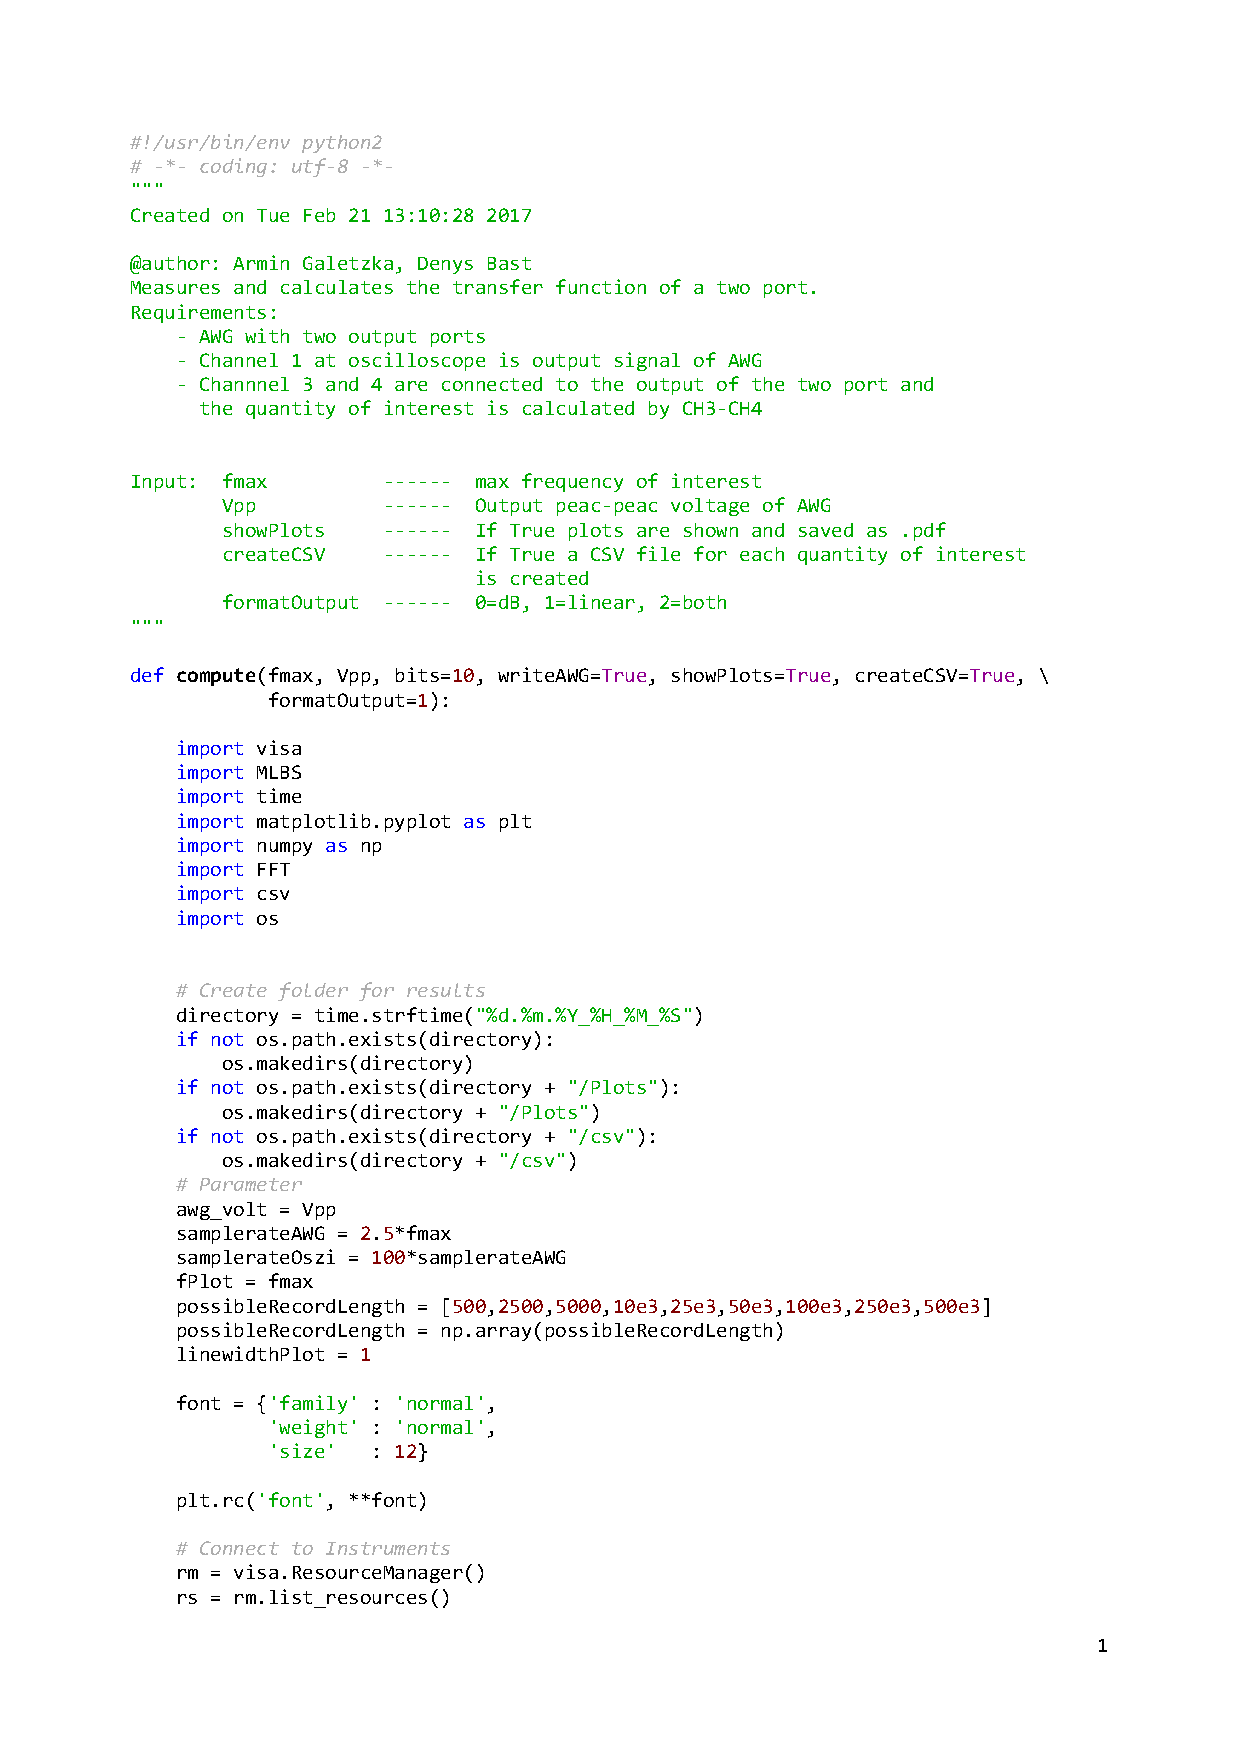
\includepdf[pages={1},noautoscale=true,scale=0.7]{Code/getH.pdf}
\end{minipage}
\includepdf[pages={2-8},noautoscale=true,scale=0.8]{Code/getH.pdf}
\subsection{MLBS.py}
\begin{minipage}[b]{0.48\linewidth} 
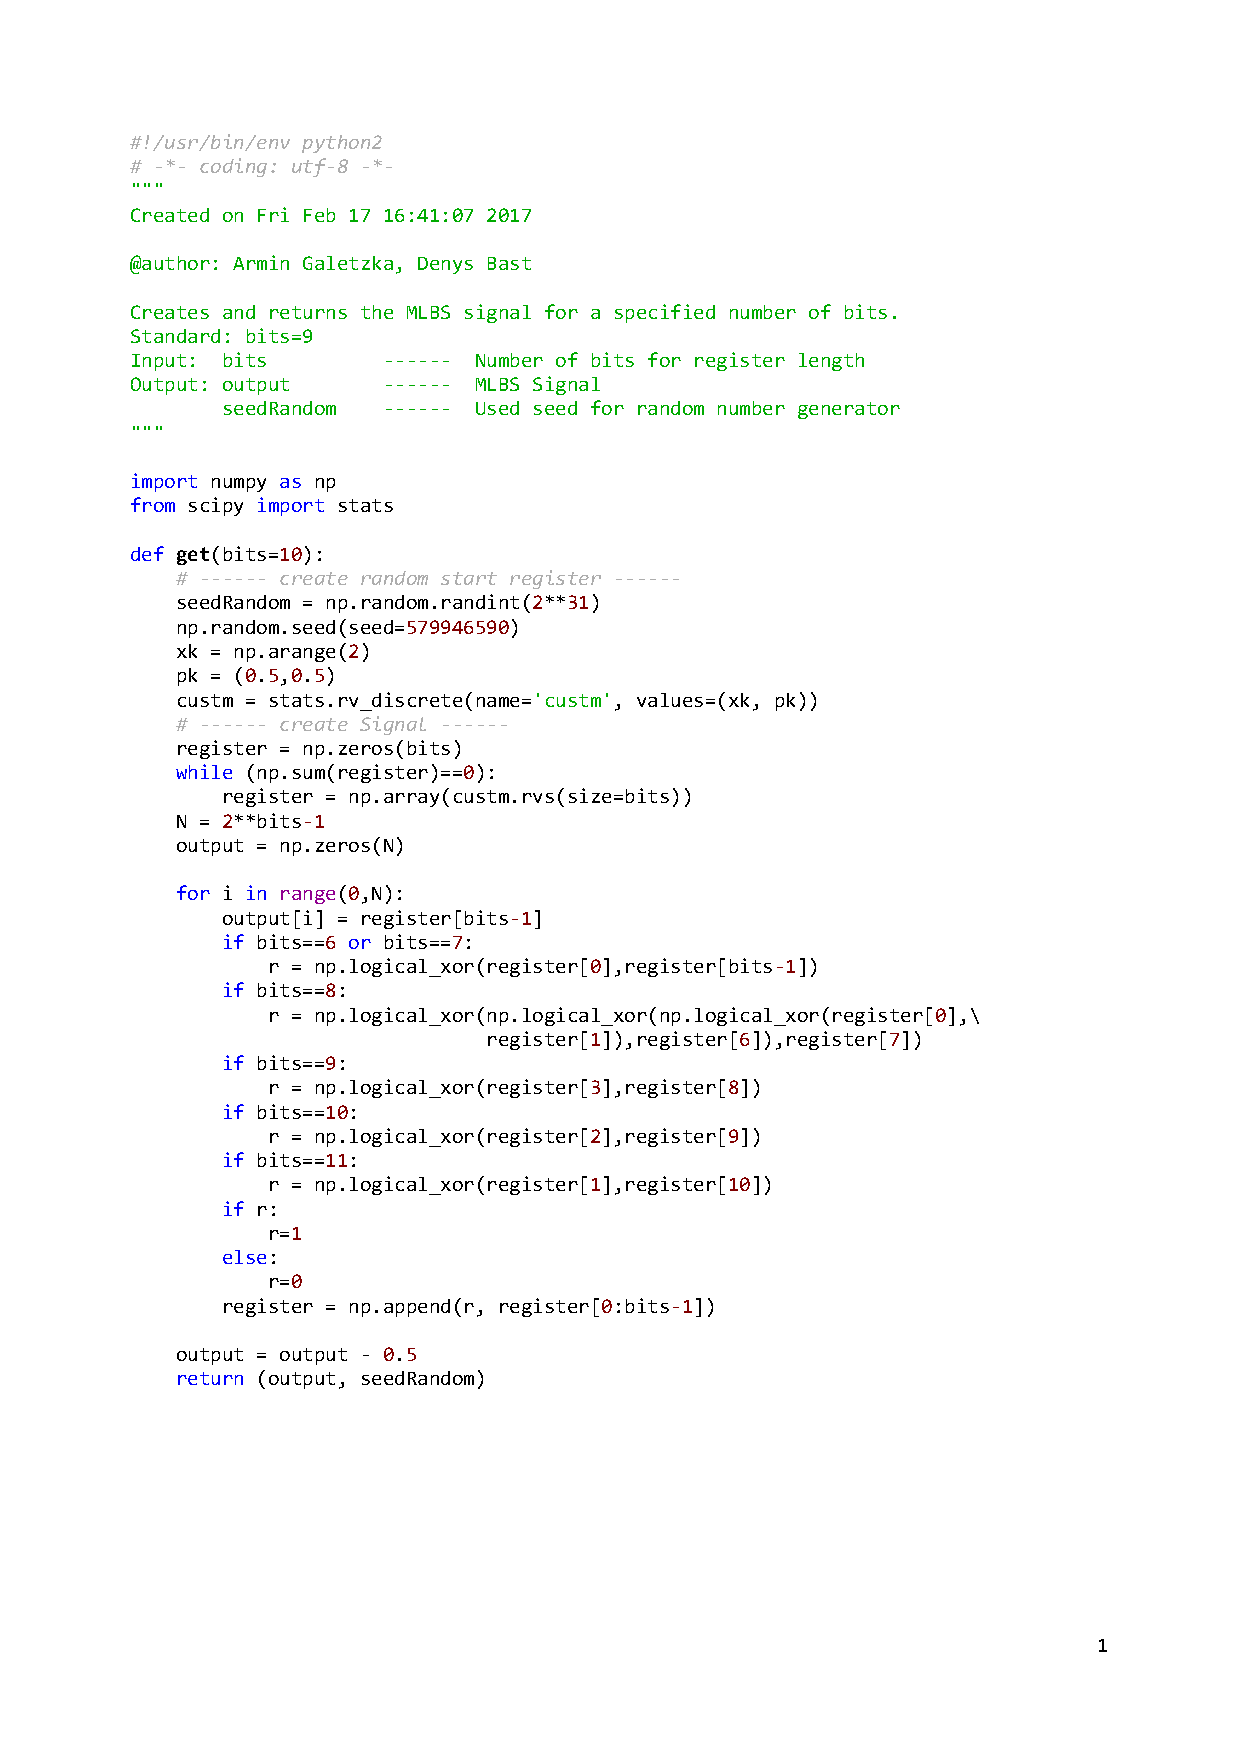
\includepdf[pages={1},noautoscale=true,scale=0.8]{Code/MLBS.pdf}
\end{minipage}
\newpage
\subsection{runme.py}
\begin{minipage}[b]{0.48\linewidth} 
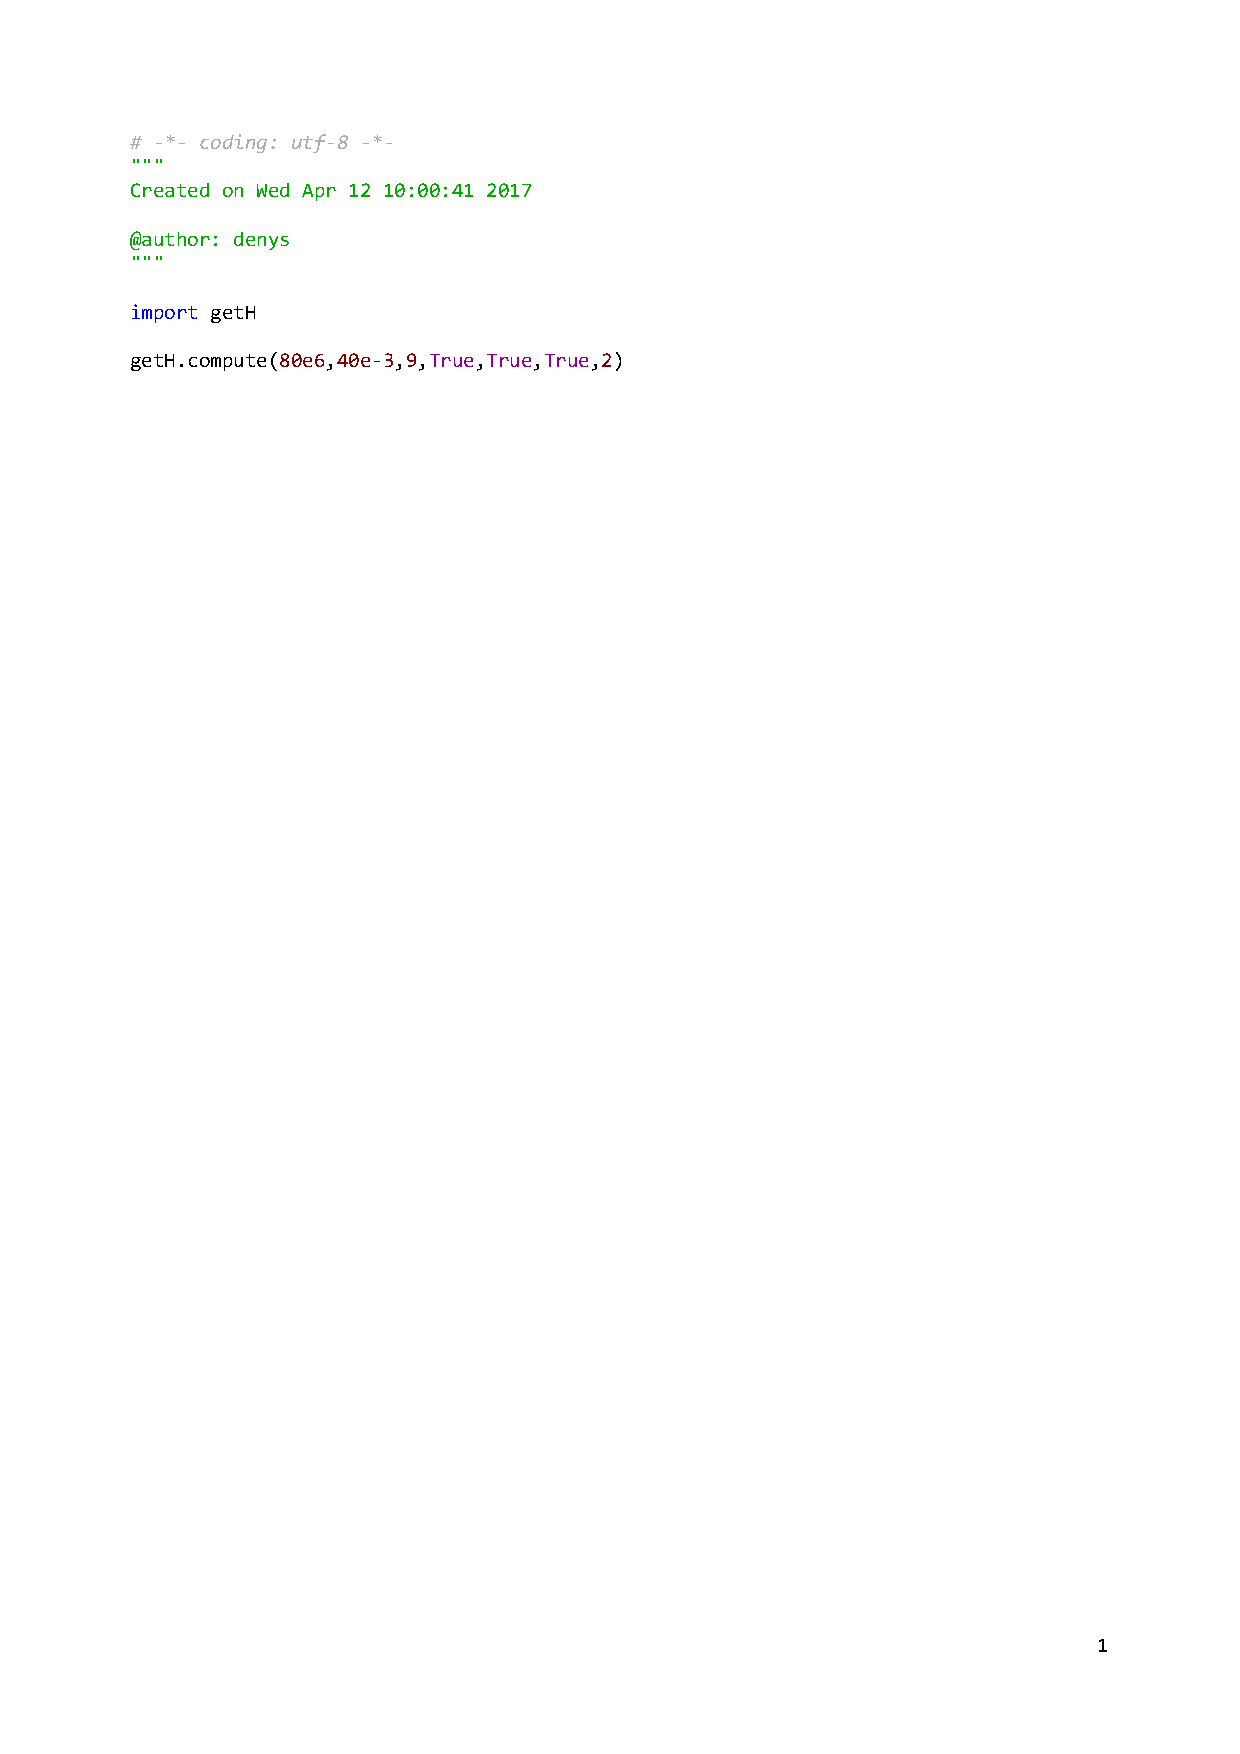
\includepdf[pages={1},noautoscale=true,scale=0.8]{Code/runme.pdf}
\end{minipage}
\newpage
\subsection{FFT.py}
\begin{minipage}[b]{0.48\linewidth} 
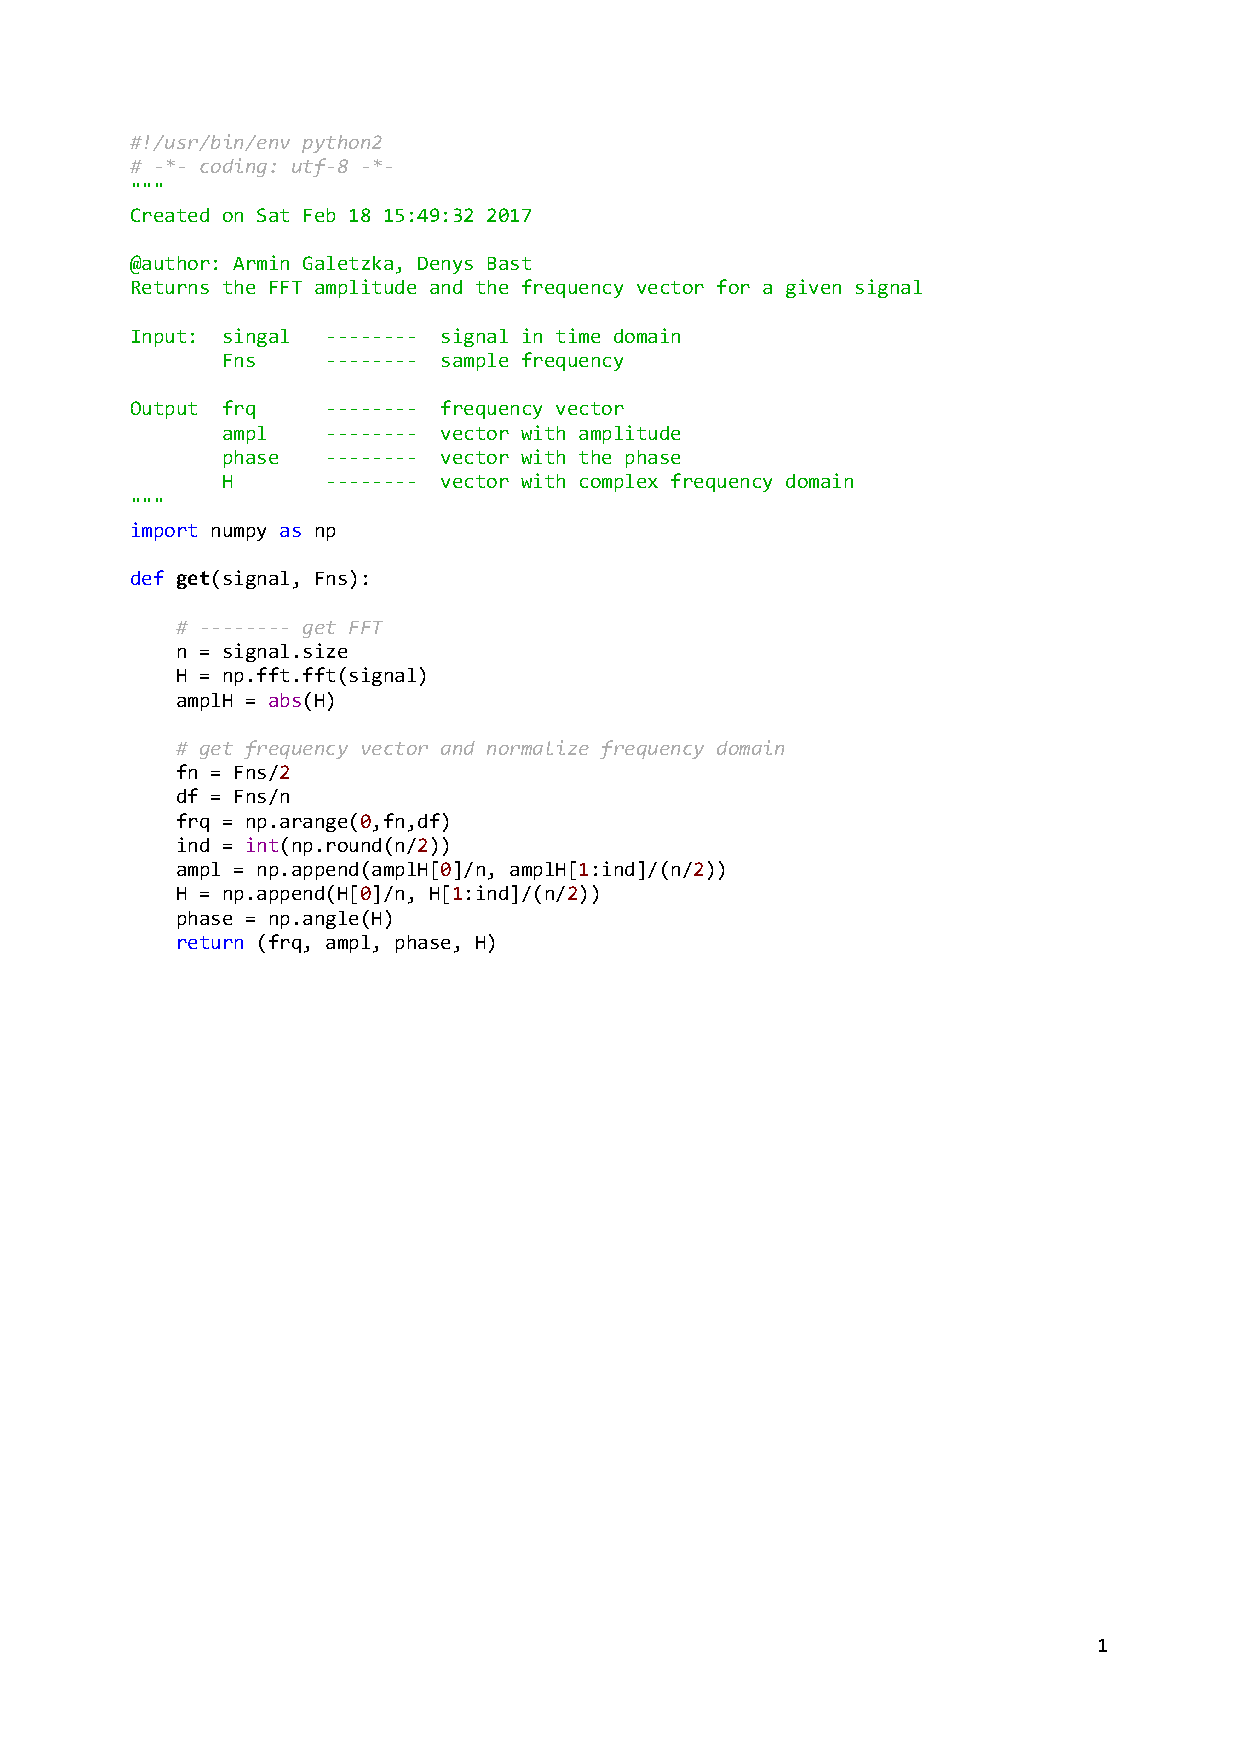
\includepdf[pages={1},noautoscale=true,scale=0.8]{Code/FFT.pdf}
\end{minipage}


\bibliography{quellen}
\end{document}